\documentclass[8pt,a4paper,compress]{beamer}

\usepackage{/home/siyer/lib/slides}

\usepackage{fancyvrb}

\newcommand{\mm}[1]{$#1$}
\newcommand{\derives}{\stackrel{*}{\Rightarrow}}

\DefineVerbatimEnvironment
{production}{Verbatim}
{fontfamily=timesroman,commandchars=\\\{\}}
\newenvironment{spaced}
{
\smallskip
\hspace{.5cm}
\begin{minipage}[c]{\textwidth}
}
{
\end{minipage}
\smallskip
}

\title{Parsing}
\date{}

\begin{document}
\begin{frame}
\vfill
\titlepage
\end{frame}

\begin{frame}
\frametitle{Outline}
\tableofcontents
\end{frame}

\section{Introduction}
\begin{frame}[fragile]
\pause

Once we have identified the tokens in our program, we then want to determine its syntactic structure and the process of doing so is called parsing

\pause
\bigskip

We wish to make sure the program is syntactically valid, ie, it conforms to the grammar that describes its syntax

\pause
\bigskip

As the parser parses the program it should identify syntax errors and report them and the line numbers they appear on

\pause
\bigskip

When the parser does find a syntax error, it should not just stop, but it should report the error, and gracefully recover so that it may go on looking for additional errors

\pause
\bigskip

The parser should produce some representation of the parsed program that is suitable for semantic analysis; in the \jmm compiler, we produce an abstract syntax tree (AST)
\end{frame}

\begin{frame}[fragile]
\pause

For example, given the following \jmm program

\begin{lstlisting}[language=Java]
package pass;

import java.lang.System;

public class Factorial {
    // Two methods and a field
    public static int factorial(int n) {
        if (n <= 0)
            return 1;
        else
            return n * factorial(n - 1);
    }
    
    public static void main(String[] args) {
        int x = n;
        System.out.println(x + "! = " + factorial(x));
    }

    static int n = 5;
}
\end{lstlisting}
we would like to produce an AST shown in the following slide
\end{frame}

\begin{frame}[fragile]
\pause

AST for the \lstinline{Factorial} program
\begin{center}
\visible<2->{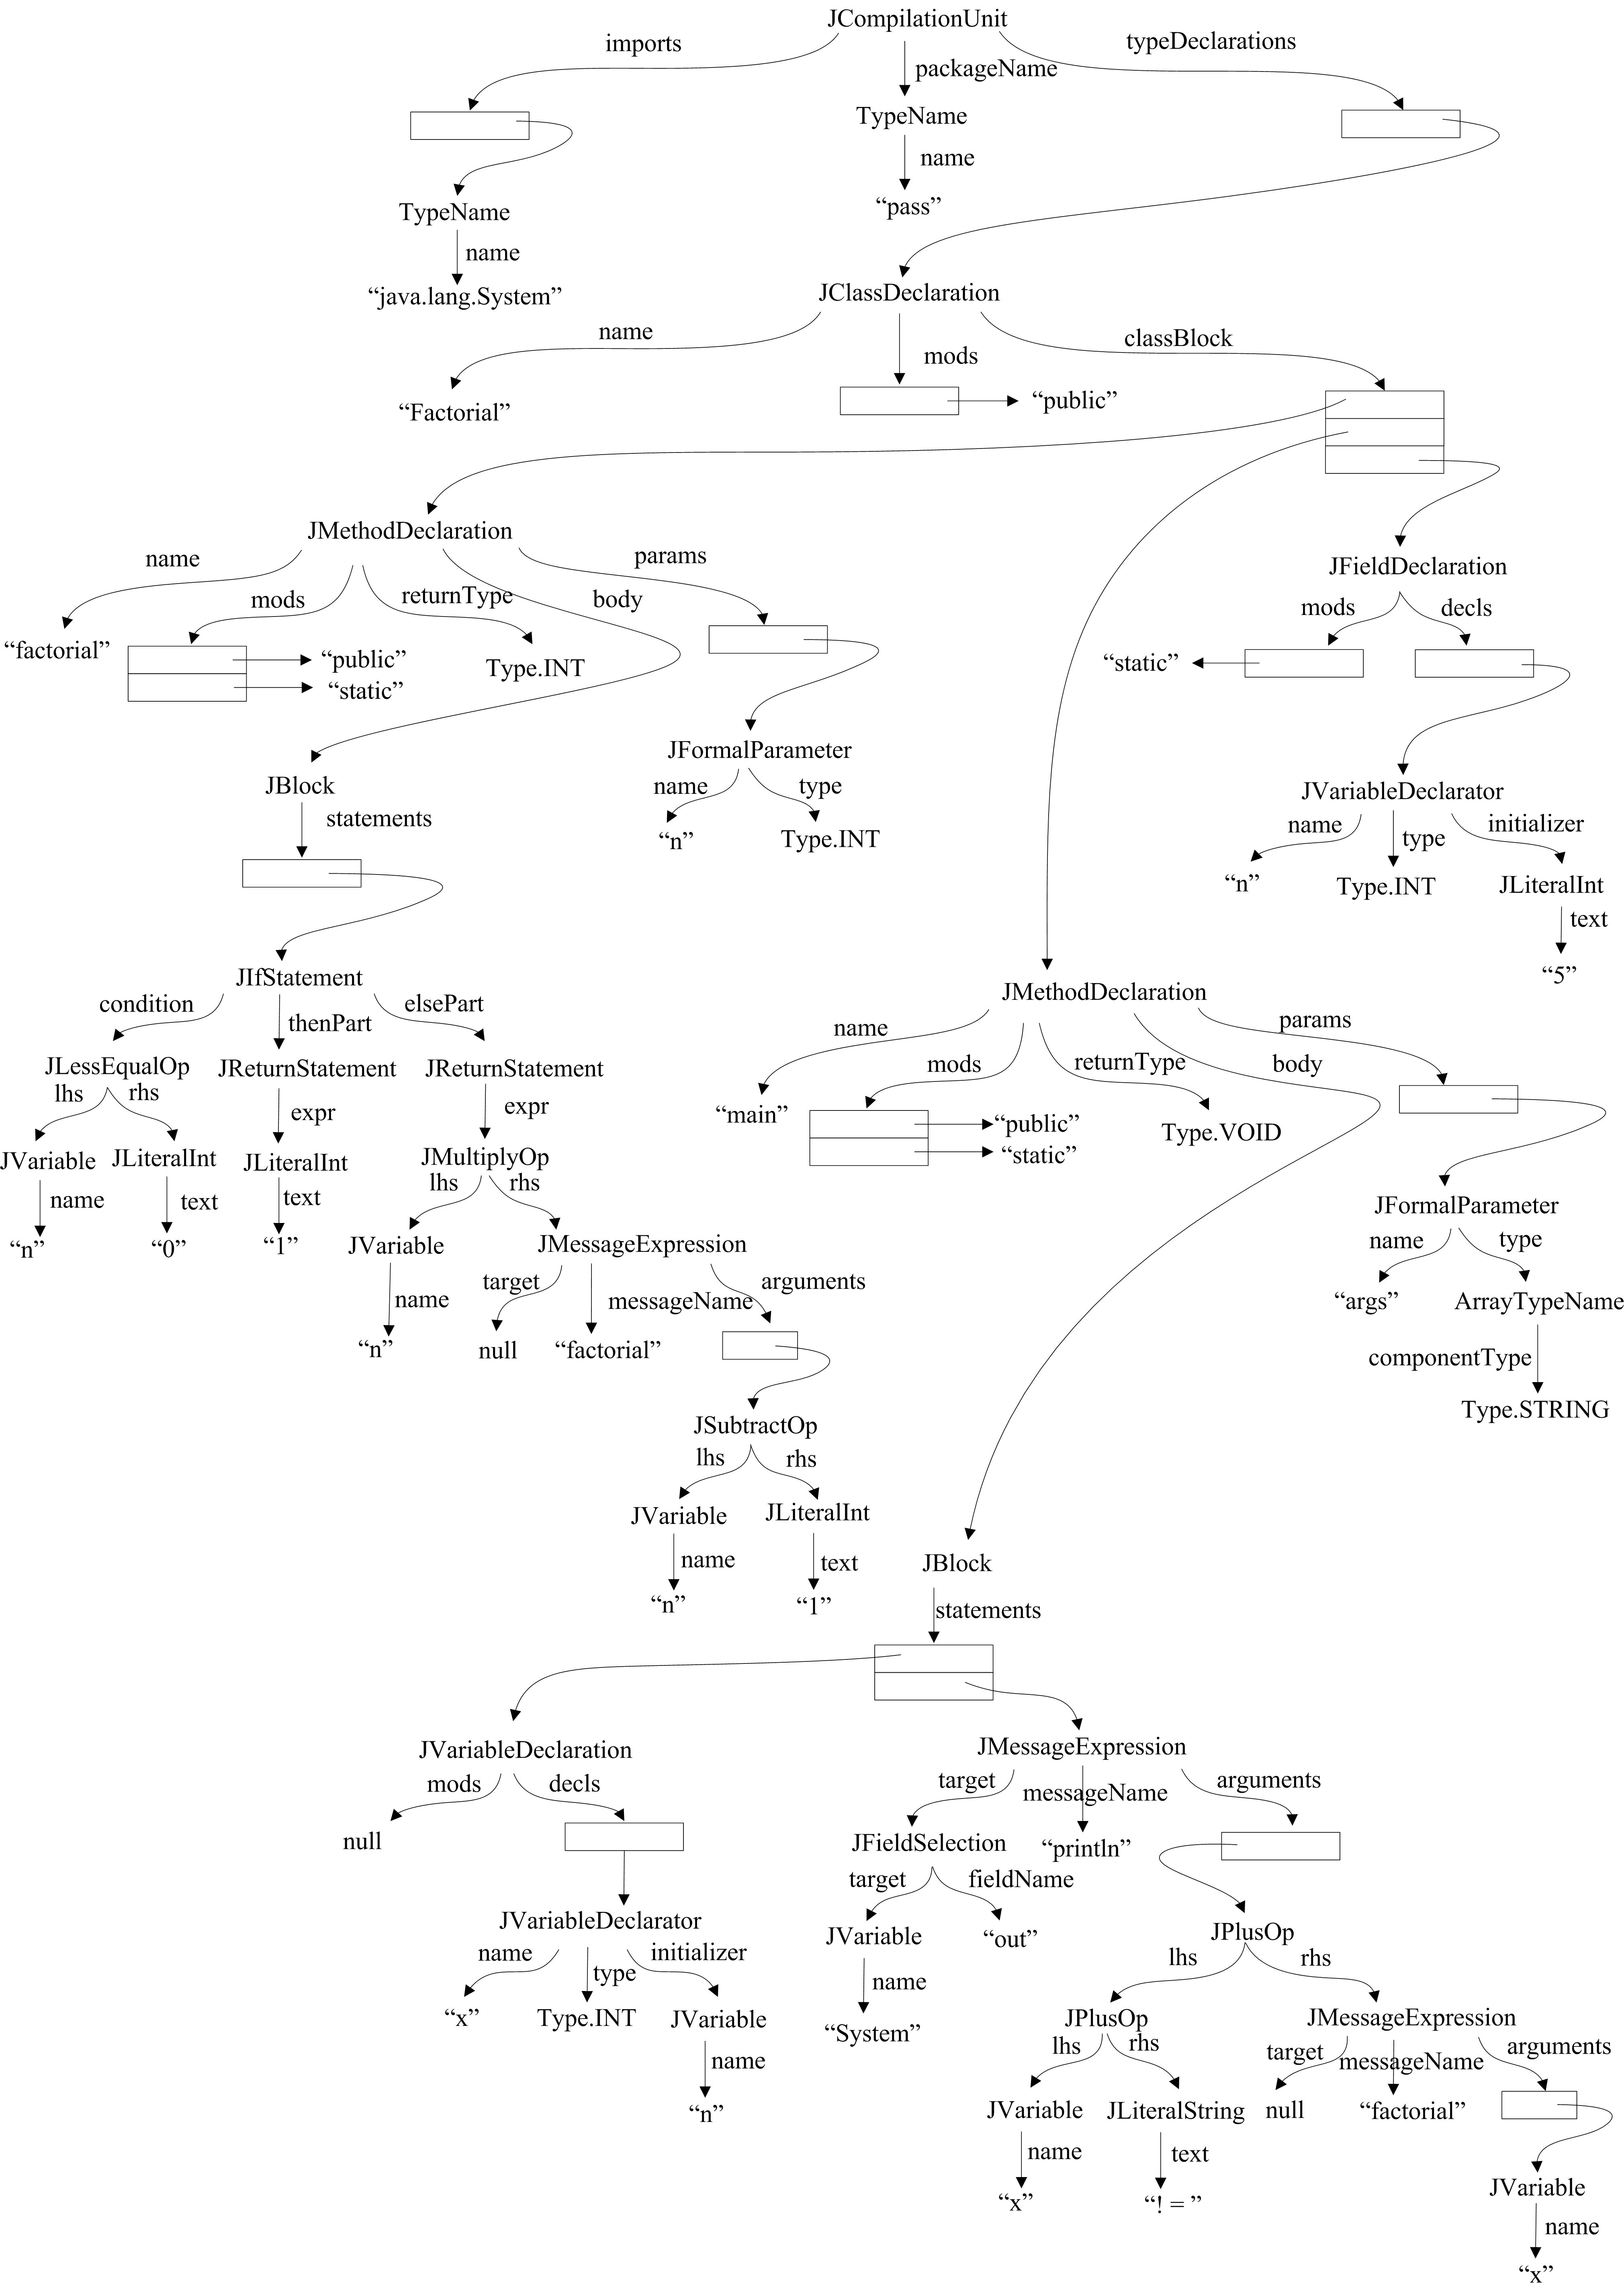
\includegraphics[scale=0.29]{{figures/figure03.01}.jpg}}
\end{center}
\end{frame}

\begin{frame}[fragile]
\pause

The nodes in the AST represent syntactic objects

\pause
\bigskip

The AST is rooted at a \lstinline{JCompilationUnit}, the syntactic object representing the program that we are compiling

\pause
\bigskip

The directed edges are labeled by the names of the fields they represent; for example, \lstinline{JCompilationUnit} has a package name, a list (an \lstinline{ArrayList}) of imported types, and a list (an \lstinline{ArrayList}) of class declarations

\pause
\bigskip

We are interested in a tree representation for our program because it is easier to analyze and decorate (with type information) a tree than it is to do the same with text

\pause
\bigskip

The AST makes the syntax implicit in the program text, explicit, which is essentially the purpose of parsing
\end{frame}

\section{Context-free Grammars and Languages}
\begin{frame}[fragile]
\pause

The grammars that we use to describe programming languages are inherently recursive and are best described by what we call context-free grammars, using a notation called Backus-Naur Form (BNF)

\pause
\bigskip

For example, the context-free rule

\text{ }
\begin{spaced}
\begin{production}
\mm{S} ::=  \lstinline{if} \lstinline{(}\mm{E}\lstinline{)} \mm{S}
\end{production}
\end{spaced}

\noindent says that, if \mm{E} is an expression and \mm{S} is a statement, then 

\text{ }
\begin{spaced}
\begin{production}
\lstinline{if} \lstinline{(}\mm{E}\lstinline{)} \mm{S}
\end{production}
\end{spaced}

\noindent is also a statement

\pause
\bigskip

There are abbreviations possible in the notation; for example, we can write

\text{ }
\begin{spaced}
\begin{production}
\mm{S} ::= \lstinline{if} \lstinline{(}\mm{E}\lstinline{)} \mm{S}
      \mm{|} \lstinline{if} \lstinline{(}\mm{E}\lstinline{)} \mm{S} \lstinline{else} \mm{S}
\end{production}
\end{spaced}

\noindent as shorthand for

\text{ }
\begin{spaced}
\begin{production}
\mm{S} ::= \lstinline{if} \lstinline{(}\mm{E}\lstinline{)} \mm{S}
\mm{S} ::= \lstinline{if} \lstinline{(}\mm{E}\lstinline{)} \mm{S} \lstinline{else} \mm{S}
\end{production}
\end{spaced}
\end{frame}

\begin{frame}[fragile]
\pause

Square brackets indicate that a phrase is optional; for example, the two rules from above can be written as

\text{ }
\begin{spaced}
\begin{production}
\mm{S} ::=  \lstinline{if} \lstinline{(}\mm{E}\lstinline{)} \mm{S} [\lstinline{else} \mm{S}]
\end{production}
\end{spaced}

\pause
\bigskip

Curly braces denote the Kleene closure, indicating that the phrase may appear zero or more times; for example

\text{ }
\begin{spaced}
\begin{production}
\mm{E} ::= \mm{T} \{\lstinline{\+} \mm{T}\}
\end{production}
\end{spaced}

\noindent says that an expression $E$ may be written as a term $T$, followed by zero or more  occurrences of \lstinline{+} followed by a term $T$, such as

\text{ }
\begin{spaced}
\begin{production}
\mm{T} \lstinline{+} \mm{T} \lstinline{+} \mm{T} \mm{\dots}
\end{production}
\end{spaced}

\pause

One may use the alternation sign $|$ inside right-hand-sides, using parentheses for grouping; for example

\text{ }
\begin{spaced}
\begin{production}
\mm{E} ::= \mm{T} \{(\lstinline{\+} \mm{|} \lstinline{\-}) \mm{T}\}
\end{production}
\end{spaced}

\noindent means that the additive operator may be either \lstinline{+} or \lstinline{-}, such as

\text{ }
\begin{spaced}
\begin{production}
\mm{T} \lstinline{+} \mm{T} \lstinline{\-} \mm{T} \lstinline{+} \mm{T}
\end{production}
\end{spaced}
\end{frame}

\begin{frame}[fragile]
\pause

BNF allows us to describe such syntax as that for a \jmm compilation unit

\text{ }
\begin{spaced}
\begin{production}
compilationUnit ::= [\lstinline{package} qualifiedIdentifier \lstinline{;}]
                           \{\lstinline{import}  qualifiedIdentifier \lstinline{;}\}
                           \{typeDeclaration\} \lstinline{EOF}
\end{production}
\end{spaced}

\pause
\bigskip

A context-free grammar\index{context-free grammar|textbf} is a tuple, $G = (N,T,S,P)$ where 
\begin{itemize}
\item $N$ is a set of non-terminal symbols, sometimes called non-terminals, 
\item $T$ is a set of terminal symbols, sometimes called terminals,
\item $S \in N$ is a designated non-terminal, called the start symbol, and
\item $P$ is a set of production rules, sometimes called productions or rules
\end{itemize}

\pause
\bigskip

For example, a context-free grammar that describes simple arithmetic expressions is $G = (N, T, S, P)$ where $N = \{E, T, F\}$ is the set of non-terminals, $T = \{\text{\lstinline{+}, \lstinline{*}, \lstinline{(}, \lstinline{)}, \lstinline{id}}\}$ is the set of terminals, $S = E$ is the start symbol, and

\text{ }
\begin{spaced}
\begin{production}
\mm{P} = \{\mm{E} ::= \mm{E} \lstinline{+} \mm{T},
        \mm{E} ::= \mm{T},
        \mm{T} ::= \mm{T} \lstinline{*} \mm{F},
        \mm{T} ::= \mm{F},
        \mm{F} ::= \lstinline{(}\mm{E}\lstinline{)},
        \mm{F} ::= \lstinline{id}\}
\end{production}
\end{spaced}
\end{frame}

\begin{frame}[fragile]
\pause

We can denote the above grammar a little less formally, simply as a sequence of production rules

\text{ }
\begin{spaced}
\begin{production}
\mm{E} ::= \mm{E} \lstinline{+} \mm{T}
\mm{E} ::= \mm{T}
\mm{T} ::= \mm{T}  \lstinline{*} {F}
\mm{T} ::= \mm{F}
\mm{F} ::= \lstinline{(}\mm{E}\lstinline{)}
\mm{F} ::= \lstinline{id}
\end{production}
\end{spaced}

\pause
\bigskip

The start symbol is important because it is from this symbol, using the production rules, that we can generate strings in a language

\pause
\bigskip

For example, we can record a sequence of applications of the production rules, starting from $E$ (starting symbol in the above grammar) to the sentence \lstinline{id + id * id} as follows

\text{ }
\begin{spaced}
\begin{production}
\mm{E} \mm{\Rightarrow} \mm{E} \lstinline{+} \mm{T}
   \mm{\Rightarrow} \mm{T} \lstinline{+} \mm{T}
   \mm{\Rightarrow} \mm{F} \lstinline{+} \mm{T}
   \mm{\Rightarrow} id \lstinline{+} \mm{T}
   \mm{\Rightarrow} id \lstinline{+} \mm{T} \lstinline{*} \mm{F}
   \mm{\Rightarrow} id \lstinline{+} \mm{F} \lstinline{*} \mm{F}
   \mm{\Rightarrow} \lstinline{id + id *} \mm{F}
   \mm{\Rightarrow} \lstinline{id + id * id}
\end{production}
\end{spaced}
\end{frame}

\begin{frame}[fragile]
\pause

When one string can be re-written as another string, using zero or more production rules from the grammar, we say the first string derives ($\derives$) the second string

\pause
\bigskip
 
For example

\text{ }
\begin{spaced}
\begin{production}
\mm{E} \mm{\derives} \mm{E} (in zero steps)
\mm{E} \mm{\derives} \lstinline{id} \lstinline{+} \mm{F} \lstinline{*} \mm{F}
\mm{T} \lstinline{+} \mm{T} \mm{\derives}  \lstinline{id + id * id}
\end{production}
\end{spaced}

\pause
\bigskip

We say the language $L(G)$ that is described by a grammar $G$ consists of all the strings (sentences) comprised of only terminal symbols, that can be derived from the start symbol, ie, $L(G) = \{w | S \derives w \text{ and } w \in T*\}$

\pause
\bigskip

For example, in the grammar above

\text{ }
\begin{spaced}
\begin{production}
\mm{E \derives} \lstinline{id + id * id}
\mm{E \derives} \lstinline{id}
\mm{E \derives} \lstinline{(id + id)} \lstinline{* id}
\end{production}
\end{spaced}

\noindent so,  $L(G)$ includes each of

\text{ }
\begin{spaced}
\begin{production}
\lstinline{id + id * id}
\lstinline{id}
\lstinline{(id + id)} \lstinline{* id}
\end{production}
\end{spaced}

\noindent and infinitely more finite sentences
\end{frame}

\begin{frame}[fragile]
\pause

We are interested in languages consisting of strings of terminals that can be derived from a grammar's start symbol

\pause
\bigskip

There are two kinds of derivation that will be important to us when we go about parsing these languages: left-most derivations and right-most derivations

\pause
\bigskip

A left-most derivation is a derivation in which at each step, the next string is derived by applying a production rule for rewriting the left-most non-terminal

\pause
\bigskip

For example

\text{ }
\begin{spaced}
\begin{production}
\underline{\mm{E}} \mm{\Rightarrow} \underline{\mm{E}} \lstinline{+} \mm{T}
   \mm{\Rightarrow} \underline{\mm{T}} \lstinline{+} \mm{T}
   \mm{\Rightarrow} \underline{\mm{F}} \lstinline{+} \mm{T}
   \mm{\Rightarrow} id \lstinline{+} \underline{\mm{T}}
   \mm{\Rightarrow} id \lstinline{+} \underline{\mm{T}} \lstinline{*} \mm{F}
   \mm{\Rightarrow} id \lstinline{+} \underline{\mm{F}} \lstinline{*} \mm{F}
   \mm{\Rightarrow} \lstinline{id + id *} \underline{\mm{F}}
   \mm{\Rightarrow} \lstinline{id + id * id}
\end{production}
\end{spaced}
\end{frame}

\begin{frame}[fragile]
\pause

A right-most derivation is a derivation in which at each step, the next string is derived by applying a production rule for rewriting the right-most non-terminal

\pause
\bigskip

For example, the right-most derivation of \lstinline{id + id * id} would go as follows

\text{ }
\begin{spaced}
\begin{production}
\underline{\mm{E}} \mm{\Rightarrow} \mm{E} \lstinline{+} \underline{\mm{T}}
   \mm{\Rightarrow} \mm{E} \lstinline{+} \mm{T} \lstinline{*} \underline{\mm{F}}
   \mm{\Rightarrow} \mm{E} \lstinline{+} \underline{\mm{T}} \lstinline{*} \lstinline{id}
   \mm{\Rightarrow} \mm{E} \lstinline{+} \underline{\mm{F}} \lstinline{*} \lstinline{id}
   \mm{\Rightarrow} \underline{\mm{E}} \lstinline{+ id * id}
   \mm{\Rightarrow} \underline{\mm{T}} \lstinline{+ id * id}
   \mm{\Rightarrow} \underline{\mm{F}} \lstinline{+ id * id}
   \mm{\Rightarrow} \lstinline{id + id * id}
\end{production}
\end{spaced}

\pause

We use the term sentential form to refer to any string of (terminal and non-terminal) symbols that can be derived from the start symbol

\pause
\bigskip

For example, in the previous derivation

\text{ }
\begin{spaced}
\begin{production}
\mm{E}
\mm{E} \lstinline{+} \mm{T}
\mm{E} \lstinline{+} \mm{T} \lstinline{*} \mm{F}
\mm{E} \lstinline{+} \mm{T} \lstinline{* id}
\mm{E} \lstinline{+} \mm{F} \lstinline{* id}
\mm{E} \lstinline{+ id * id}
\mm{T} \lstinline{+ id * id}
\mm{F} \lstinline{+ id * id}
\lstinline{id + id * id}
\end{production}
\end{spaced}
\end{frame}

\begin{frame}[fragile]
\pause

An alternative representation of a derivation is the parse tree, a tree that illustrates the derivation and the structure of an input string (at the leaves) from a start symbol (at the root)

\pause
\bigskip

For example, the following figure shows the parse tree for \lstinline{id + id * id}.

\begin{center}
\visible<3->{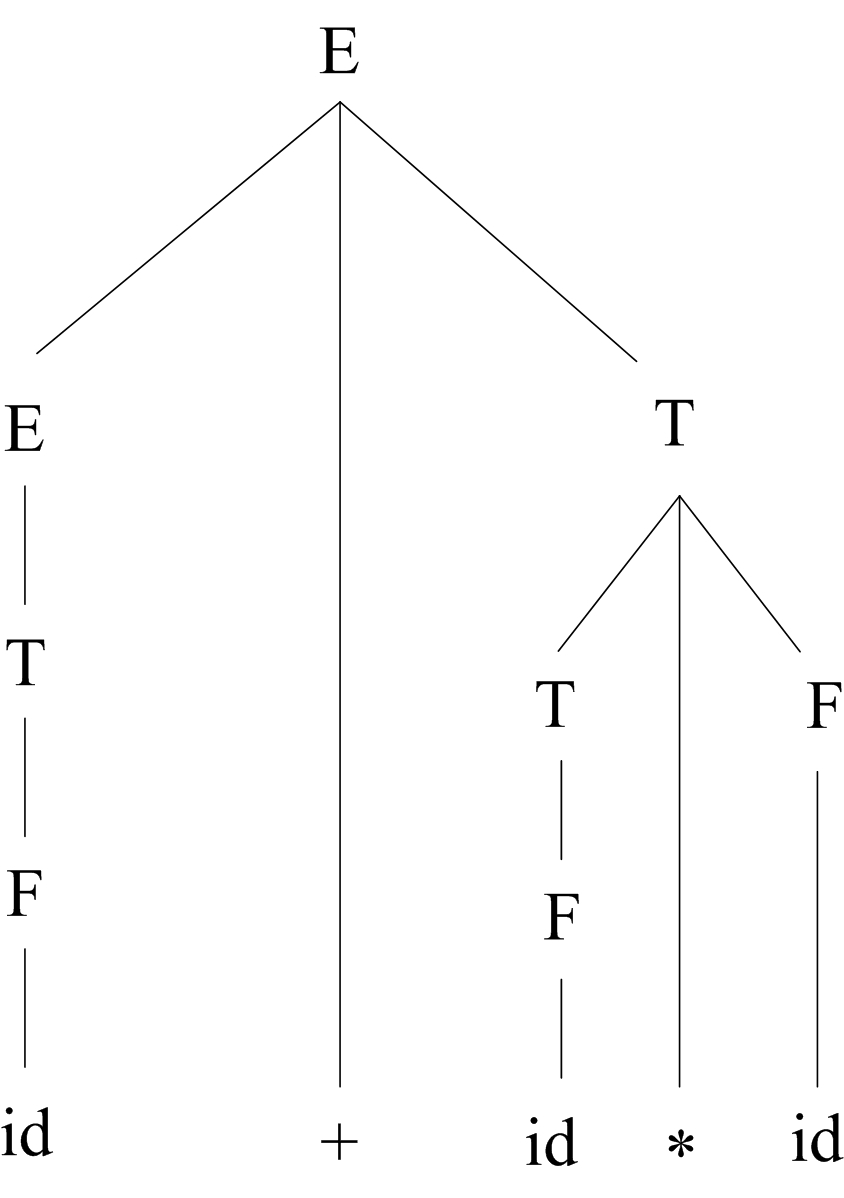
\includegraphics[scale=0.6]{{figures/figure03.02}.jpg}}
\end{center}

\pause
\bigskip

Given a grammar $G$, if there exists a sentence $s$ in $L(G)$ for which there are more than one left-most derivations in $G$ (or equivalently, either more than one right-most derivations, or more than one parse tree for $s$ in $G$), we say that the sentence $s$ is ambiguous

\pause
\bigskip

If a grammar $G$ describes at least one ambiguous sentence, the grammar $G$ is an ambiguous grammar; if there is no such sentence, we say the grammar is unambiguous
\end{frame}

\begin{frame}[fragile]
\pause

Consider the grammar

\text{ }
\begin{spaced}
\begin{production}
\mm{E} ::= \mm{E} \lstinline{+} \mm{E} \mm{|} \mm{E} \lstinline{*} \mm{E} \mm{|} \lstinline{(}\mm{E}\lstinline{)} \mm{|} \lstinline{id}
\end{production}
\end{spaced}

\noindent and, consider the sentence \lstinline{id + id * id}

\pause
\bigskip

One left-most derivation for this sentence is

\text{ }
\begin{spaced}
\begin{production}
\underline{\mm{E}} \mm{\Rightarrow} \underline{\mm{E}} \lstinline{+} \mm{E}
   \mm{\Rightarrow} \lstinline{id +} \underline{\mm{E}}
   \mm{\Rightarrow} \lstinline{id +} \underline{\mm{E}} \lstinline{*} \mm{E}
   \mm{\Rightarrow} \lstinline{id + id *} \underline{\mm{E}}
   \mm{\Rightarrow} \lstinline{id + id * id}
\end{production}
\end{spaced}

\pause
\bigskip

Another left-most derivation of the same sentence is

\text{ }
\begin{spaced}
\begin{production}
\underline{\mm{E}} \mm{\Rightarrow} \underline{\mm{E}} \lstinline{*} \mm{E}
   \mm{\Rightarrow} \underline{\mm{E}} \lstinline{+} \mm{E} \lstinline{*} \mm{E}
   \mm{\Rightarrow} \lstinline{id +} \underline{\mm{E}} \lstinline{*} \mm{E}
   \mm{\Rightarrow} \lstinline{id + id *} \underline{\mm{E}}
   \mm{\Rightarrow} \lstinline{id + id * id}
\end{production}
\end{spaced}

\pause
\bigskip

Therefore, the grammar is ambiguous
\end{frame}

\begin{frame}[fragile]
\pause

The above sentence also has two right-most derivations in the grammar

\text{ }
\begin{spaced}
\begin{production}
\underline{\mm{E}} \mm{\Rightarrow} \mm{E} \lstinline{+} \underline{\mm{E}}
   \mm{\Rightarrow} \mm{E} \lstinline{+} \mm{E} \lstinline{*} \underline{\mm{E}}
   \mm{\Rightarrow} \mm{E} \lstinline{+} \underline{\mm{E}} \lstinline{* id}
   \mm{\Rightarrow} \underline{\mm{E}} \lstinline{+ id * id}
   \mm{\Rightarrow} \lstinline{id + id * id}
\end{production}
\end{spaced}

\noindent and

\text{ }
\begin{spaced}
\begin{production}
\underline{\mm{E}} \mm{\Rightarrow} \mm{E} \lstinline{*} \underline{\mm{E}}
   \mm{\Rightarrow} \underline{\mm{E}} \lstinline{* id}
   \mm{\Rightarrow} \mm{E} \lstinline{+} \underline{\mm{E}} \lstinline{* id}
   \mm{\Rightarrow} \underline{\mm{E}} \lstinline{+ id * id}
   \mm{\Rightarrow} \lstinline{id + id * id}
\end{production}
\end{spaced}

\noindent with the following two parse trees
\begin{center}
\visible<2->{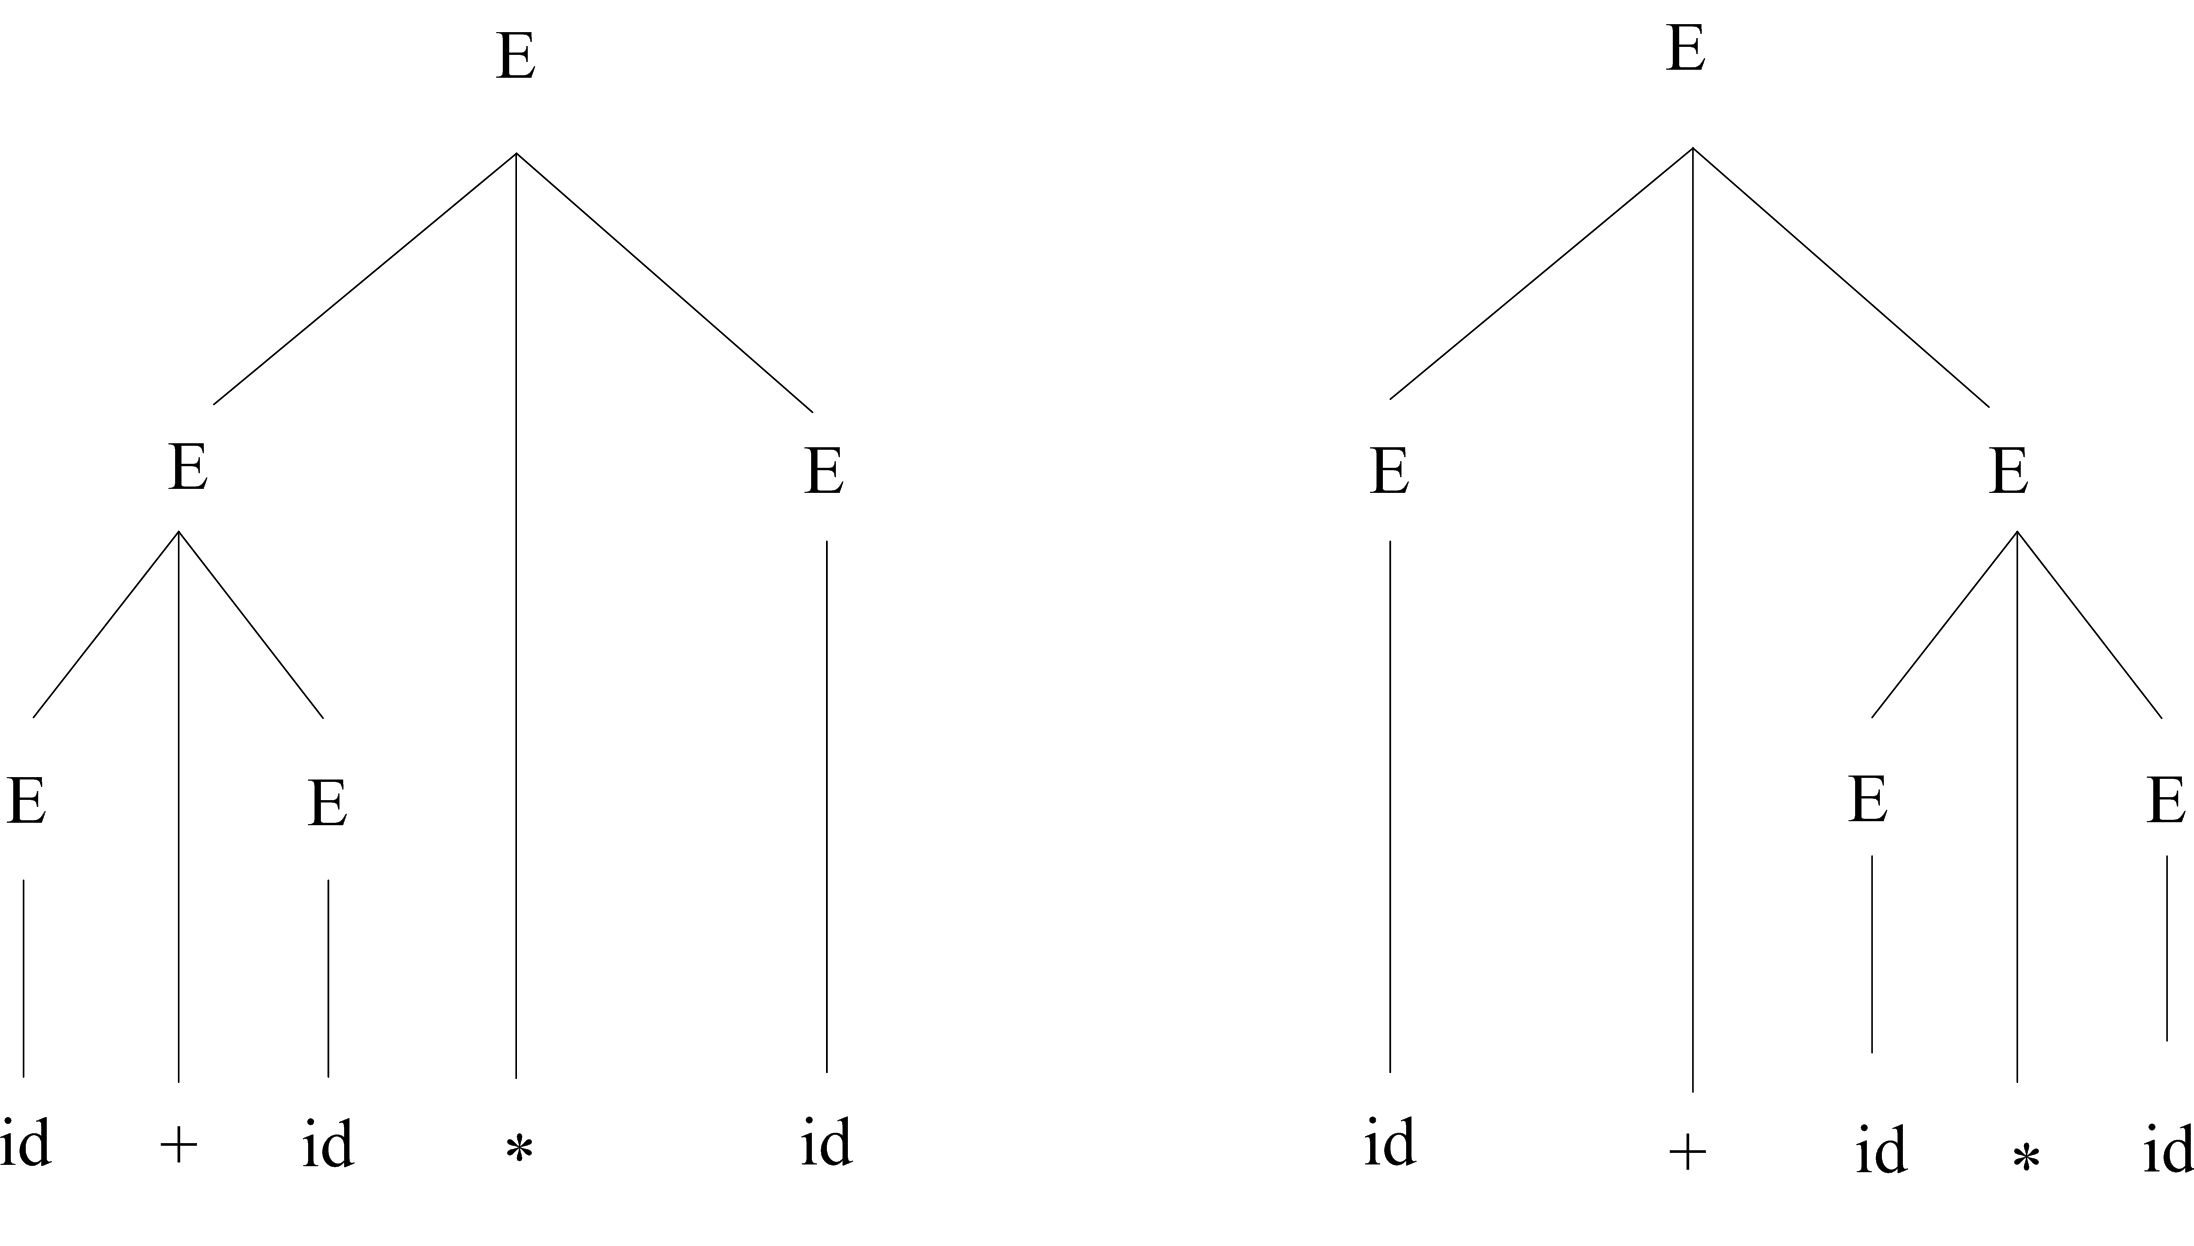
\includegraphics[scale=0.4]{{figures/figure03.03}.jpg}}
\end{center}
\end{frame}

\begin{frame}[fragile]
\pause

As another example, consider the grammar describing conditional statements

\text{ }
\begin{spaced}
\begin{production}
\mm{S} ::= \lstinline{if} \lstinline{(}\mm{E}\lstinline{)} \mm{S}
      \mm{|} \lstinline{if} \lstinline{(}\mm{E}\lstinline{)} \mm{S} \lstinline{else} \mm{S}
      \mm{|} \lstinline{s}
\mm{E} ::=  \lstinline{e}
\end{production}
\end{spaced}

and consider the sentence

\text{ }
\begin{spaced}
\begin{production}
\lstinline{if (e)} \lstinline{if (e)} \lstinline{s else s}
\end{production}
\end{spaced}
\end{frame}

\begin{frame}[fragile]
\pause

There exist two left-most derivations for the above sentence in the grammar

\text{ }
\begin{spaced}
\begin{production}
\underline{\mm{S}} \mm{\Rightarrow} \lstinline{if} \lstinline{(}\underline{\mm{E}}\lstinline{)} \mm{S} \lstinline{else} \mm{S}
   \mm{\Rightarrow} \lstinline{if} \lstinline{(e)} \underline{\mm{S}} \lstinline{else} \mm{S}
   \mm{\Rightarrow} \lstinline{if} (e) \lstinline{if} \lstinline{(}\underline{\mm{E}}\lstinline{)} \mm{S} \lstinline{else} \mm{S}
   \mm{\Rightarrow} \lstinline{if} (e) \lstinline{if} \lstinline{(e)} \underline{\mm{S}} \lstinline{else} \mm{S}
   \mm{\Rightarrow} \lstinline{if} \lstinline{(e)} \lstinline{if} \lstinline{(e) s} \lstinline{else} \underline{\mm{S}}
   \mm{\Rightarrow} \lstinline{if} \lstinline{(e)} \lstinline{if} \lstinline{(e) s} \lstinline{else} \lstinline{s}
\end{production}
\end{spaced}

\noindent and

\text{ }
\begin{spaced}
\begin{production}
\underline{\mm{S}} \mm{\Rightarrow} \lstinline{if} \lstinline{(}\underline{\mm{E}}\lstinline{)} \mm{S}
   \mm{\Rightarrow} \lstinline{if} \lstinline{(e)} \underline{\mm{S}}
   \mm{\Rightarrow} \lstinline{if} \lstinline{(e)} \lstinline{if} \lstinline{(}\underline{\mm{E}}\lstinline{)} \mm{S} \lstinline{else} \mm{S}
   \mm{\Rightarrow} \lstinline{if} \lstinline{(e)} \lstinline{if} \lstinline{(e)} \underline{\mm{S}} \lstinline{else} \mm{S}
   \mm{\Rightarrow} \lstinline{if} \lstinline{(e)} \lstinline{if} \lstinline{(e)} \lstinline{s} \lstinline{else} \underline{\mm{S}}
   \mm{\Rightarrow} \lstinline{if} \lstinline{(e)} \lstinline{if} \lstinline{(e) s} \lstinline{else} \lstinline{s}
\end{production}
\end{spaced}

\noindent with the following parse trees

\begin{center}
\visible<2->{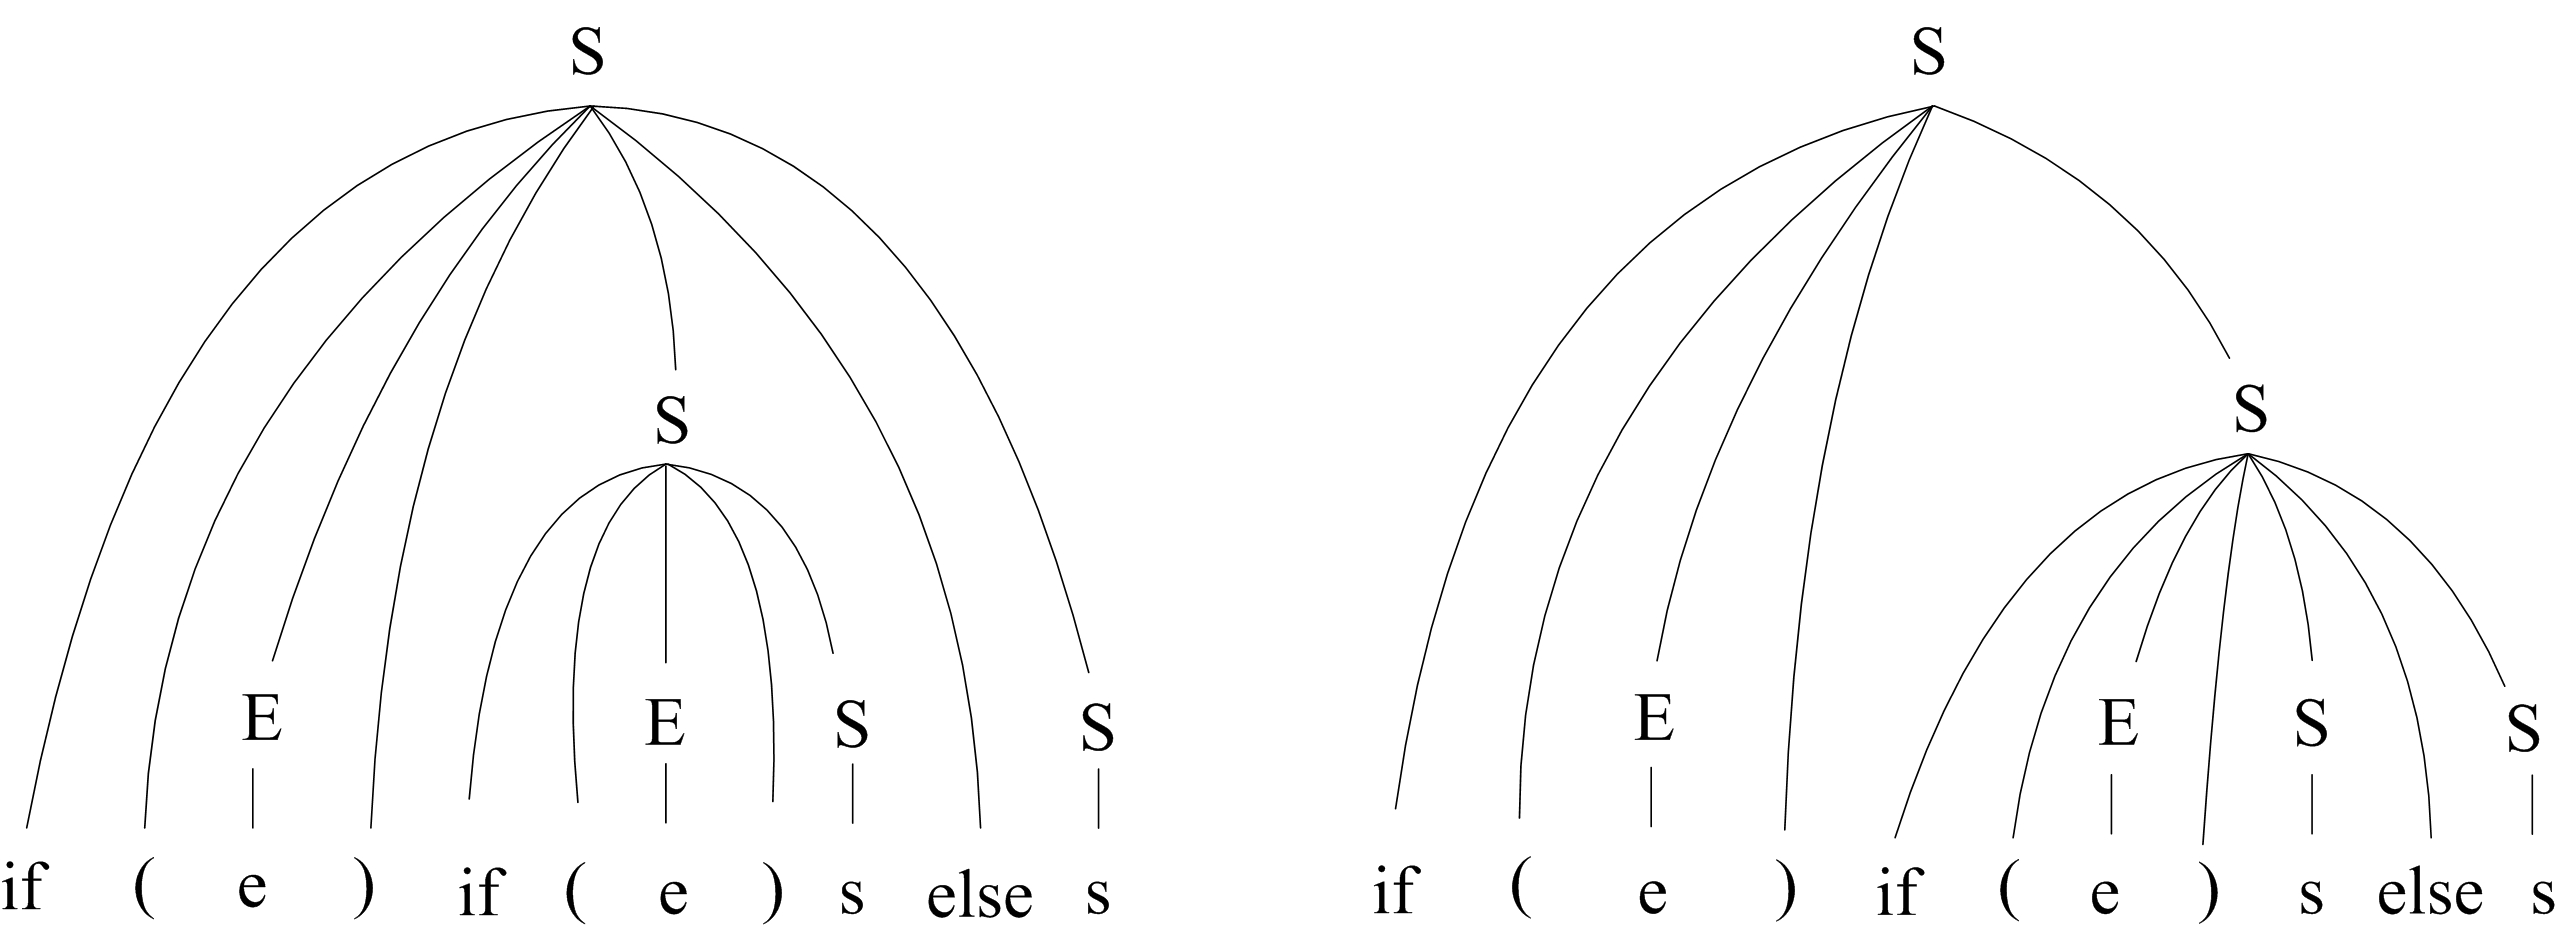
\includegraphics[scale=0.4]{{figures/figure03.04}.jpg}}
\end{center}
\end{frame}

\begin{frame}[fragile]
\pause

One could easily modify the syntax of conditionals to remove the ambiguity

\text{ }
\begin{spaced}
\begin{production}
\mm{S} ::= \lstinline{if} \mm{E} \lstinline{do} \mm{S}
      \mm{|} \lstinline{if} \mm{E} \lstinline{then} \mm{S} \lstinline{else} \mm{S}
      \mm{|} \lstinline{s}
\mm{E} ::= \lstinline{e}
\end{production}
\end{spaced}

\pause
\bigskip

But programmers have become both accustomed to (and fond of) the ambiguous conditional

\pause
\bigskip

Compiler writers handle the rule as a special case in the compiler's parser, making sure that an \lstinline{else} is grouped along with the closest preceding \lstinline{if}.
\end{frame}

\begin{frame}[fragile]
\pause

The \jmm grammar (and the Java grammar) have another ambiguity, which is even more difficult; consider the problem of parsing the expression \lstinline{x.y.z.w}

\pause
\bigskip

Clearly \lstinline{w} is a field; if it were a method expression, then that would be evident in the syntax \lstinline{x.y.z.w()}

\pause
\bigskip

But, what about \lstinline{x.y.z}?  There are several possibilities depending on the types of the names \lstinline{x}, \lstinline{y} and \lstinline{z}

\begin{itemize}
\item If \lstinline{x} is the name of a local variable, it might refer to an object with a field \lstinline{y}, referring to another object with a field \lstinline{z}, referring to yet another object having our field \lstinline{w}; in this case, the expression would be parsed as a cascade of field selection expressions

\item Alternatively, \lstinline{x.y} might be the name of a package, in which the class \lstinline{z} is defined; in this case, we would parse the expression by first parsing \lstinline{x.y.z} as a fully qualified class and then parse \lstinline{w} as a static field selection of that class

\item Other possibilities, parsing various permutations of (possibly qualified) class names and field selection operations, also exist
\end{itemize}

\pause
\bigskip

The parser cannot determine how the expression \lstinline{x.y.z} is parsed because types are not decided until after it has parsed the program and constructed its AST, so represents \lstinline{x.y.z} in the AST by an \lstinline{AmbiguousName} node; later on, after type declarations have been processed, the compiler re-writes this node as the appropriate sub-tree
\end{frame}

\section{Top-down Deterministic Parsing}
\begin{frame}[fragile]
\pause

\end{frame}

\section{Bottom-up Deterministic Parsing}
\begin{frame}[fragile]
\pause

\end{frame}

\section{Parser Generation Using JavaCC}
\begin{frame}[fragile]
\pause

\end{frame}
\end{document}
